\section{Theoretical model}
\label{mod_pres}
% ou presenter Warren et DDM : dans background et motivation ? Ici ?

%We now introduce our theoretical model. We remind that 
%Our goal is to conceive a turn-taking model for an embodied conversational agent engaged in a dyadic interaction with the user, namely a mixed-initiative dialog. 
%To reach this goal we divided the conception of our model in several steps. We first elaborated our theoretical model based on these assumptions and did a first validation step by comparing the results of agent-agent simulations to real human interactions. Then, we implemented our model in a computational agent architecture and evaluated the behavior of our agent in real-time interactions with the user. 

%In this section we specifically present our theoretical model. We will expose in the next section an analysis of the model properties and the comparison between agent-agent simulations and user-agent simulation, how we implemented our model in a computational agent architecture and how we tested the behavior of our agent in the context of real-time interactions with the user. 

%We begin by introducing our model, starting with the assumptions we made about the behavior of our agent, then describing more in details our theoretical model. 

\subsection{Overall architecture}

Concerning the turn-taking management, depending of their current role in the conversation, the goals of the agents are as follows: being the current speaker, the agent's goals are to give the turn or to keep it; being the current listener, its goals are to take the turn or to go on listening. Whatever their current role (speaker or listener) the agents actively, indeed proactively, produce verbal and nonverbal signals accordingly to their current goal. 
The signals they produced also drive their behavior. For instance, in a given context, the current listener will start to speak, if it has something to say, and when it will observe a variation in the signals produced by the current speaker indicating that it is about to end its turn. 
Thus, at any moment of time, and maybe at the same time, the agents have to decide whether they want to change their role or not (transitioning from speaker to listener or conversely). However, the agents will not directly perform the corresponding communicative actions because they also take into account the behavior of the other agents. 
Finally the time when the turn will actually change results in the complex interplay of the individual behavior of each agents. Moreover, this individual behavior is controlled by two cognitive processes: the first one controls the agent's own motivation to change its role; the second one controls the production of the communicative signals. 
Figure \ref{fig:mot} presents the two levels of dynamics implied in the control of the agent's behavior.

%Before describing in details our model we want to clarify the distinction we made between the different cognitive processes implied in turn-taking management. The figure \ref{mot} presents the two levels of dynamics implied in the control of the agent's behavior.

\begin{figure}
  \centering
  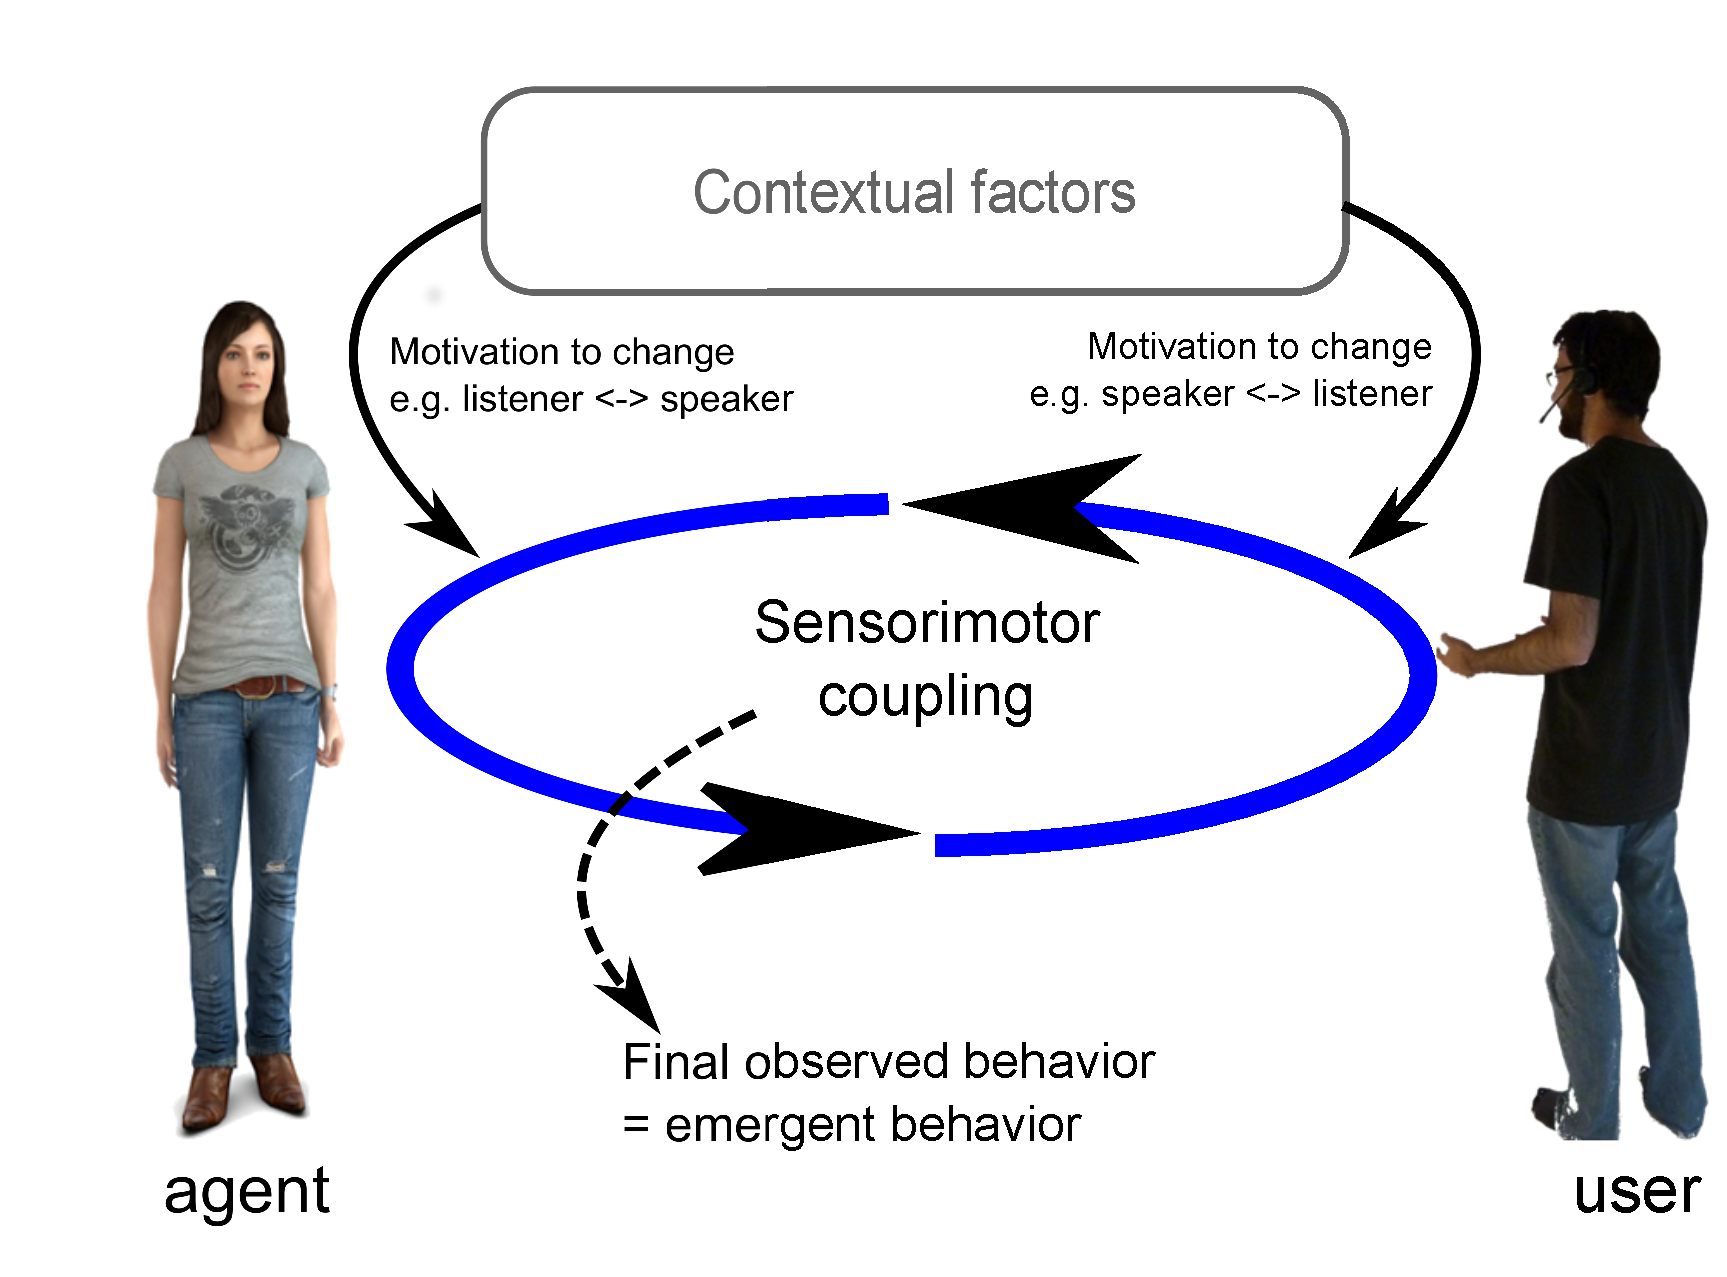
\includegraphics[width=\linewidth]{figure/schema_motivation.eps}

  \caption{The two levels of dynamics involved in the turn-taking management. 
    Top level: the contextual factors, like the verbal productions, and the interpersonal attitudes, vary the motivation the each agent has in the current situation to change its role (being the speaker or the listener). 
Bottom level: the coordination process itself, partly driven by the agent's motivation and partly resulting from the sensorimotor coupling between the two participants. 
The observed behavior of the agents is an emergent property resulting from the interplay of the agents' behavior.}
  \label{fig:mot}
\end{figure}
% the Distinction between the motivation to speak driven by contextual factors like verbal content, and interpersonal attitudes, and the coordination process itself partly driven by the motivation of the participants and emergent from the sensorimotor coupling between participants.}

The first level at the top of the figure represents the contextual factors that impact how the agents tries to take, release or keep the turn. These contextual factors are numerous. Examples of these variables are the nature of the verbal contribution, especially the importance the contribution has towards the progression of the dialog \citep{selfridge_bidding_2009}, its competitive or cooperative nature \citep{cafaro_effects_2016}, or the agent's attitude towards its partner \citep{ter_maat_how_2010}. 
These factors influence, or modulate, the ``motivation'' of the agent to claim the turn when it is the current listener or to release the turn when it is the current speaker. 
In other words, these factors define the relative strength of the goals of each agent, namely changing its role (speaker, listener) or still keeping it. It is worth noticing that this motivation continuously varies during the interaction. 
%In our model, these factors do not directly traduce into ``strategies" \citep{ter_maat_how_2010} or complete actions the agent will make towards the coordination of speaking turn but will more simply modulate the ``motivation'' the agent has to change its role (transitioning from speaker to listener or conversely). 
What we call here ``motivation" is similar to what other authors have called ``urge to speak" \citep{thorisson_multiparty_2010} or ``intentions"  to speak \citep{lessmann_towards_2004}, in the sense that it represents a variable that modulates the strength with which the agent will try to take or release the turn. We chose to call it ``motivation'' to remain as neutral as possible towards the contextual factors that could modulate this variable, as for example, taking the turn early is not always related to an urgency to say something, and is not always related to explicit communicative intentions, as participant's emotions and attitudes can also impact the agent's behavior. 

In the  model, this motivation is a variable that continuously varies between $-1$ and $1$. 
$-1$ means that the agent has a strong motivation to keep its current role (listening or speaking), while
$1$ means that the agent has a strong motivation to adopt the opposite role. 
%Between these two values the agent can continuously vary the strength with which it will try to keep or change its role, 
The closer the value of the motivation to $0$ the weaker the strength of the participant to change its role or to keep it. 

The value of the motivation influences, but does not solely determine, the final behavior of the agent in terms of taking, yielding or keeping the turn. The motivation variable represents the goal of the agent towards turn-taking, but the final behavior of the agent is an emergent property of the interaction between the agent and its partner. 
This principle results from the second loop of interaction in Figure \ref{mot}. 
In this loop, the agent begins to vary its own signals regarding turn-taking (for example, decreasing loudness or pitch or gaze towards the user) based on its own goal as conveyed by the motivation variable. Nevertheless, the agent is coupled with its partner, and the signal production of its interlocutor directly influences the way it will vary its own signals.
Conversely the variation of its own actions will influence the behavior of its partner. 
As a result, the final behavior of the agent
%, either the participant will take, yield or keep the turn and the shape of this behavior 
is an emergent property of the interaction between the participants.
It results from the complex interplay between the own motivation of the participant and the cues given by its interlocutor.

\subsection{Scope of the modelling}

The objective of this study is the modeling of the continuous sensorimotor coupling between the participants. In this context, the motivation of the agent acts as a control parameter of the dynamics of this coupling. Thus the law of control of this motivation is out of the scope of this work.
%In our model, we suppose that the motivation value is influenced by different contextual variables as presented here, but we only interested for the moment in the modeling
Moreover, our aim here is not to define the law of control for the production of the verbal and nonverbal signals, as observed in human conversations, but to model the general dynamics of the behavior and thus to capture the way these various signals shape the agent's behavior. For the sake of generality, in the presentation of the theoretical model, we consider abstract values of these signals and their variations are simplified in purpose, compared to what can be observed in human conversations.
%exactly the signals produced in human conversations, but to model the more general dynamics of the signals produced by participants. The signal values taken as example here are then theoretical and their evolution is voluntarily simplified compared to human conversations. 
For instance, the different prosodic features are treated as continuous variables, whereas is human conversations their dynamics are linked to the phonemes produced by the participants. More precisely, the model accounts for the suprasegmental evolution of the prosodic signals, which is primarily linked to the coordination of turns.
% that's why we chose to abstract here from the part of the prosody that is correlated with the verbal content of what the user says. 
The same principle is followed for other signals mentioned in this article like gestures or gaze directions. 
Another reason for this abstraction % of the signals perceived and produced by the model is that our goal is to create a generic
is to make the  theoretical model independent to the actual sensors and actuators that could be used for real-time interactions between the agent and the user. 
We will see in section \ref{impl} the capacity of our implementation to adapt to real interactive setup, and will explain more in details how we used our theoretical values to modulate the prosody of the text-to-speech system.

\subsection{Components of the theoretical model}

We will now introduce in details our theoretical model, which is divided in two components as shown in Figure \ref{fig:mod-comp}: one in charge of the continuous perception of the user's behavior and one that controls the production of the different communicative signals. 

\begin{figure}
  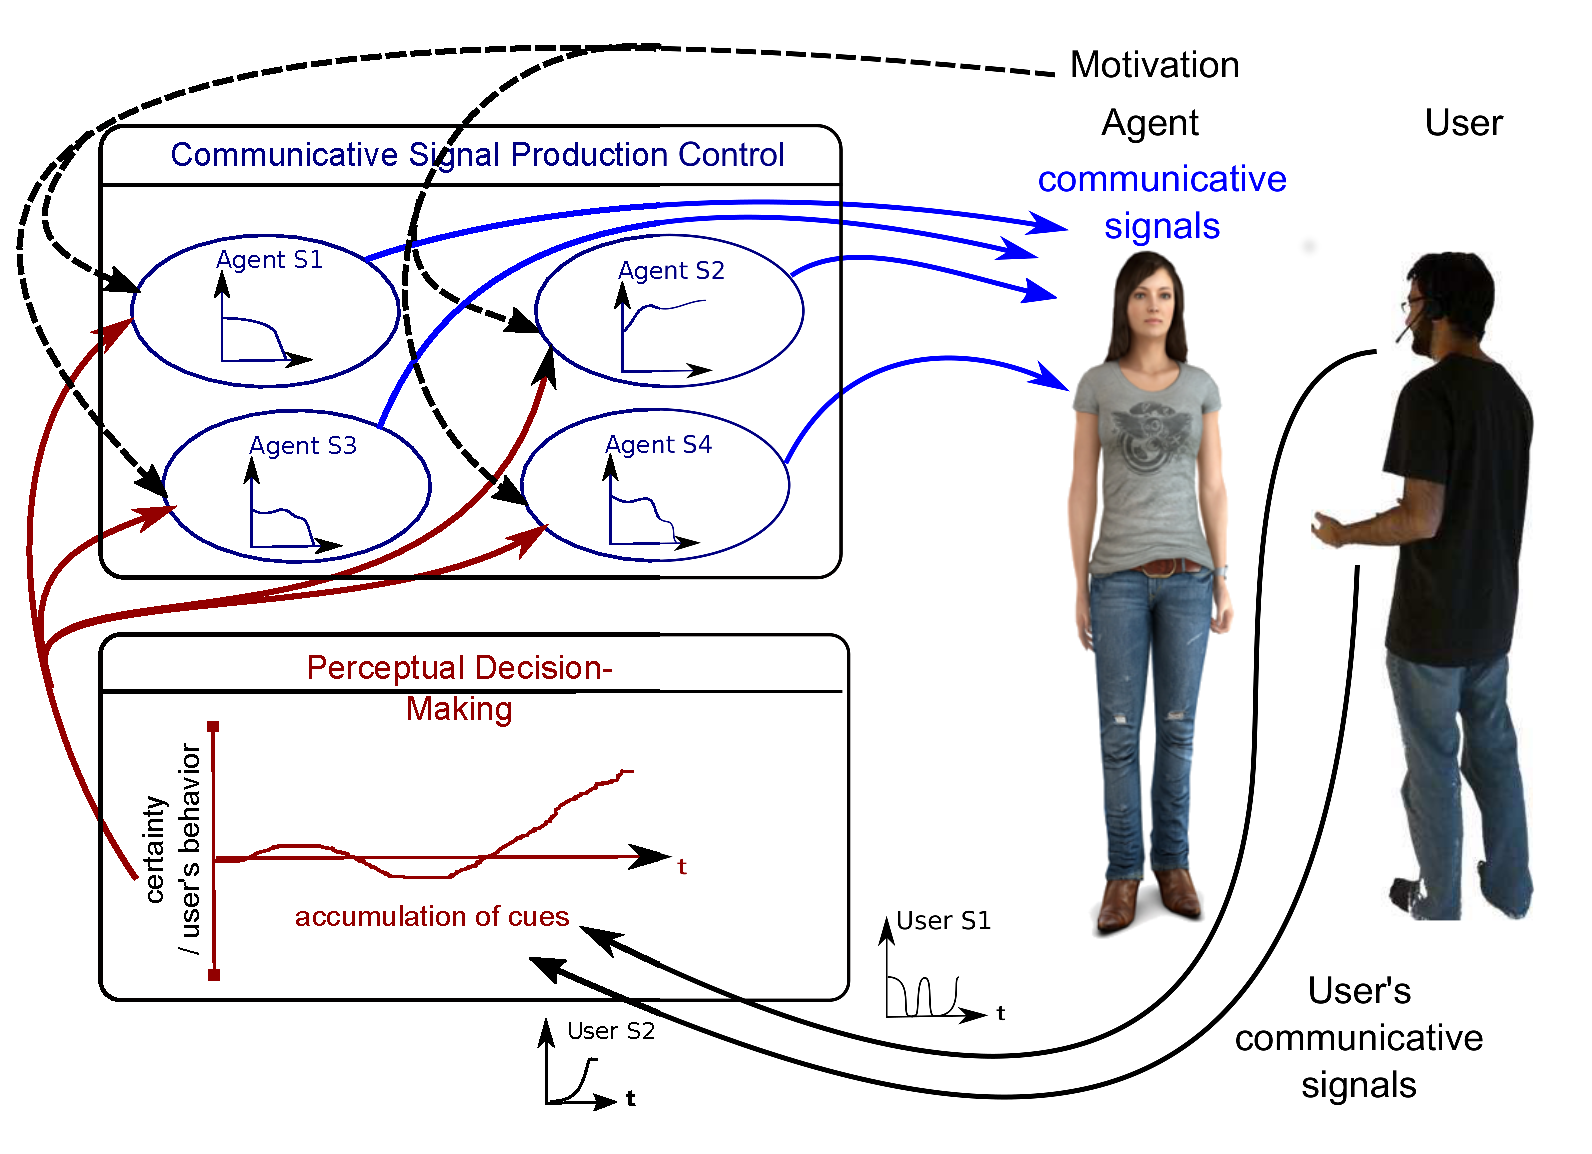
\includegraphics[width=\linewidth]{figure/modele_conceptuel_act.eps}
  \caption{Overview of Components of the theoretical model.}
  \label{fig:mod-comp}
\end{figure}

%First the agent tries to perceive the current behavior of the user between two alternatives, whether the user is changing role or not that is to say, whether the user is taking the turn or listening, if the agent is the current speaker or either the user is yielding or not the turn if the agent is the current listener. The agent continuously perceives the variations of the user signals over time, and continuously updates an accumulation variable that represents the degree of certainty the agent has about the user's behavior. 
%Second, the agent continuously modulates his nonverbal signals, based on the accumulation variable computed in the user behavior perception component and the agent's own motivation to change role. The way the agent controls his nonverbal signals is defined by a set of deterministic differential equations, where both accumulation and motivation are used to compute the attractors of the equations, that is, the final value towards which converge the agent signals.  

%We will now present more in details the different components of our model.

\subsubsection{Perceptual decision-making}
%\subsubsection{User behavior perception}

This component accounts for the dynamics of the decision-making. The underlying cognitive process is a perceptual decision-making task. The agent continuously perceives the variations of the signals produced by the user during the interaction, and continuously evaluates its certainty about the willingness of the user to be the next speaker (or listener). This degree of certainty is represented by an accumulation variable (see Figure \ref{fig:mod-comp}).
The user behavior perception component follows the paradigm of Two Alternative Forced Choice tasks (TAFC), for which different solutions have been proposed in order to model the timing of the decision making process (see \citep{bogacz_physics_2006} for a review). 
The Drift Diffusion Model (DDM) has been one of the mostly. It has shown its ability to predict the time required by a human subject to accurately discriminate the nature of the information it can perceive. 
Interestingly the DDM have been used both in settings where the stimuli presented to the subject remained the same over the course of the decision-making process and settings where the stimuli varied \cite{ratcliff_note_1980}. This model conceptualizes the dynamics of the agent's decision-making as a stochastic process driven by the following equation:

\begin{equation}
  \frac{d\gamma(t)}{dt}=\alpha(t)+c\times\frac{dW}{dt}
  \label{perc_int}
\end{equation}

In our model, Equation \ref{perc_int}, $\gamma(t)$ represents the current degree of certainty the agent has about the behavior of its partner, $\alpha(t)$ an accumulation rate that varies depending on the continuous variations of the user's signals and $c\times\frac{dW}{dt}$ representing a noise in the perception process of the participants as defined by the DDM. The decision making process is therefore continuously driven by the perception of the signals produced by the agent's partner.

%Depending on 
The sign of $\gamma(t)$ indicates that the agent is tending to adopt one alternative or the other. 
When $\gamma(t)>0$, the higher its value, the more the agent is certain about its partner's willingness to switch to the opposite role.
When $\gamma(t)<0$, a high absolute value means that the agent is very certain that its partner actually wants to keep its current role. 

The ongoing decision-making process ends when $\gamma(t)$ crosses a threshold $\theta_{\gamma}^{\pm}$. $\gamma(t)$ is then set to 0 and a new decision making process starts.
$\gamma(t) \geq theta_{\gamma}^{+}$ means that the agent is certain that its partner has switch to the opposite role and the agent changes its behavior accordingly (defined by the component responsible for the control of signals). $\gamma(t) \leq theta_{\gamma}^{-}$ means that the signals it can perceive indicate that its partner wants to keep its current role. 
%When $\gamma(t)>0$, the agent is more or less certain about the fact that its partner wants to change role, that is, if the partner is giving or yielding the turn. When  $\gamma(t)<0$, the agent is more or less certain about the fact that its partner wants to change role. 

%When $\gamma(t)$ crosses a threshold $\theta_{\gamma}^{\pm}$, favoring one or the other alternative, it means that the agent becomes certain about the nature of the behavior of its partner, either the partner changes role $\theta_{\gamma}^{+}$ or keep its current role $\theta_{\gamma}^{-}$. When the accumulation value crosses the threshold $\theta_{\gamma}^{+}$, the agent changes its own role. As a consequence, the agent activates the corresponding behavior (defined by the component responsible for the control of signals) and initialize a new perceptual decision-making task, corresponding to its newly adopted role.
%as  modifying the equations controlling its nonverbal signals and the user behavior perception equation. 

%On the opposite, when $\gamma(t)$ crosses the threshold $\theta_{\gamma}^{-}$, the agent resets its accumulation value, forgetting what it has perceived before and beginning a new perceptual decision-making process. 
We will see in section \ref{mod_analysis}, that reinitializing this accumulation value allows, for instance, the agent motivated to take or to yield the turn to try to initiate a new turn transition if the previous try did not succeed. 
It occurs when its partner does not respond to its turn-yielding signals by taking the turn, or when the agent's partner being the current speaker, prevents the agent to take the turn.

To account for the sensorimotor coupling between the two agents, we made the accumulation rate $\alpha(t)$ being a function of the variations of the signals produced by the agent's partner. This function has a general shape defined by the equation: 

\begin{equation}
  \alpha(t) = \sum_{j=0}^{n_{s}} \alpha_{j}(\dot{s}_j(t),s_j(t))
  \label{alpha_func}
\end{equation}

Equation \ref{alpha_func} means that $\alpha(t)$ continuously varies according to a sum of partial accumulation processes $\alpha_{j}$ that compute an accumulation rate for each signal $s_j$ the agent can perceive ($n_s$ denotes the number of signals). %of the agent's partner. 
$\alpha_{j}>0$ indicates that the current variations in the signals produced by its partner are in favor of the assumption that the partner is switching to  the opposite role.
$\alpha_{j}<0$  means that the perceived variations of the signals are in favor of the assumption that the partner is keeping its current role. 
%$n_{s}$ represents the number of signals of the user. 

\paragraph{Illustrative simulation S1.}% To illustrate the  perceptual decision-making process, 
Let's consider a situation with an agent able to perceive the variations of loudness, pitch, and gaze direction of the user, three cues that are considered as used by participants to coordinate their turns (see section \ref{backgd}). 
%For gesture, we refer to gesticulations as defined by \citep{duncan_signals_1972} as the production of gestures without referring to the meaning of these gesture. 
% TODO
In this simulated interaction, the agent was the current speaker and the user the current listener. The behavior of the user was here simulated.
%The user is initiating some gesticulations, slowly increasing their speed over time, then 
The user averted its gaze after 750~ms and started to speak at $t=1~s$. %take the turn at about 1~s. 
Figures \ref{fig-volume-user1}, \ref{fig-pitch-user1} and \ref{fig-gaze-user1} illustrate the variations of the simulated user's signal production, as perceived by the agent. 
We forced the agent to never leave the turn (its motivation to keep the turn was constant and maximal $m = -1$).
%varies his signals as presented in figure \ref{part_actions}. It represents a user beginning to initiate gesticulations 
Figure \ref{acc_example} illustrates the resulting dynamics of the perceptual decision-making process. 
%In this scenario, the agent is the current speaker and a simulated user tries to take the turn by varying its signals according to figure \ref{part_actions}. 
The curve at the top is the evolution of the accumulation rate over time, $\frac{d\gamma(t)}{dt}$ and the curve at the bottom the evolution of the accumulation value $\gamma(t)$. 

% TODO: subfigures

% \begin{figure}
% \centering
% \includegraphics[width=\linewidth]{figure/Gesticulation_speed_partenaire.pdf}
% \caption{Gesture production speed of the simulated user.}
% \label{part_gesture}
% \end{figure}

\begin{figure}
  \centering
  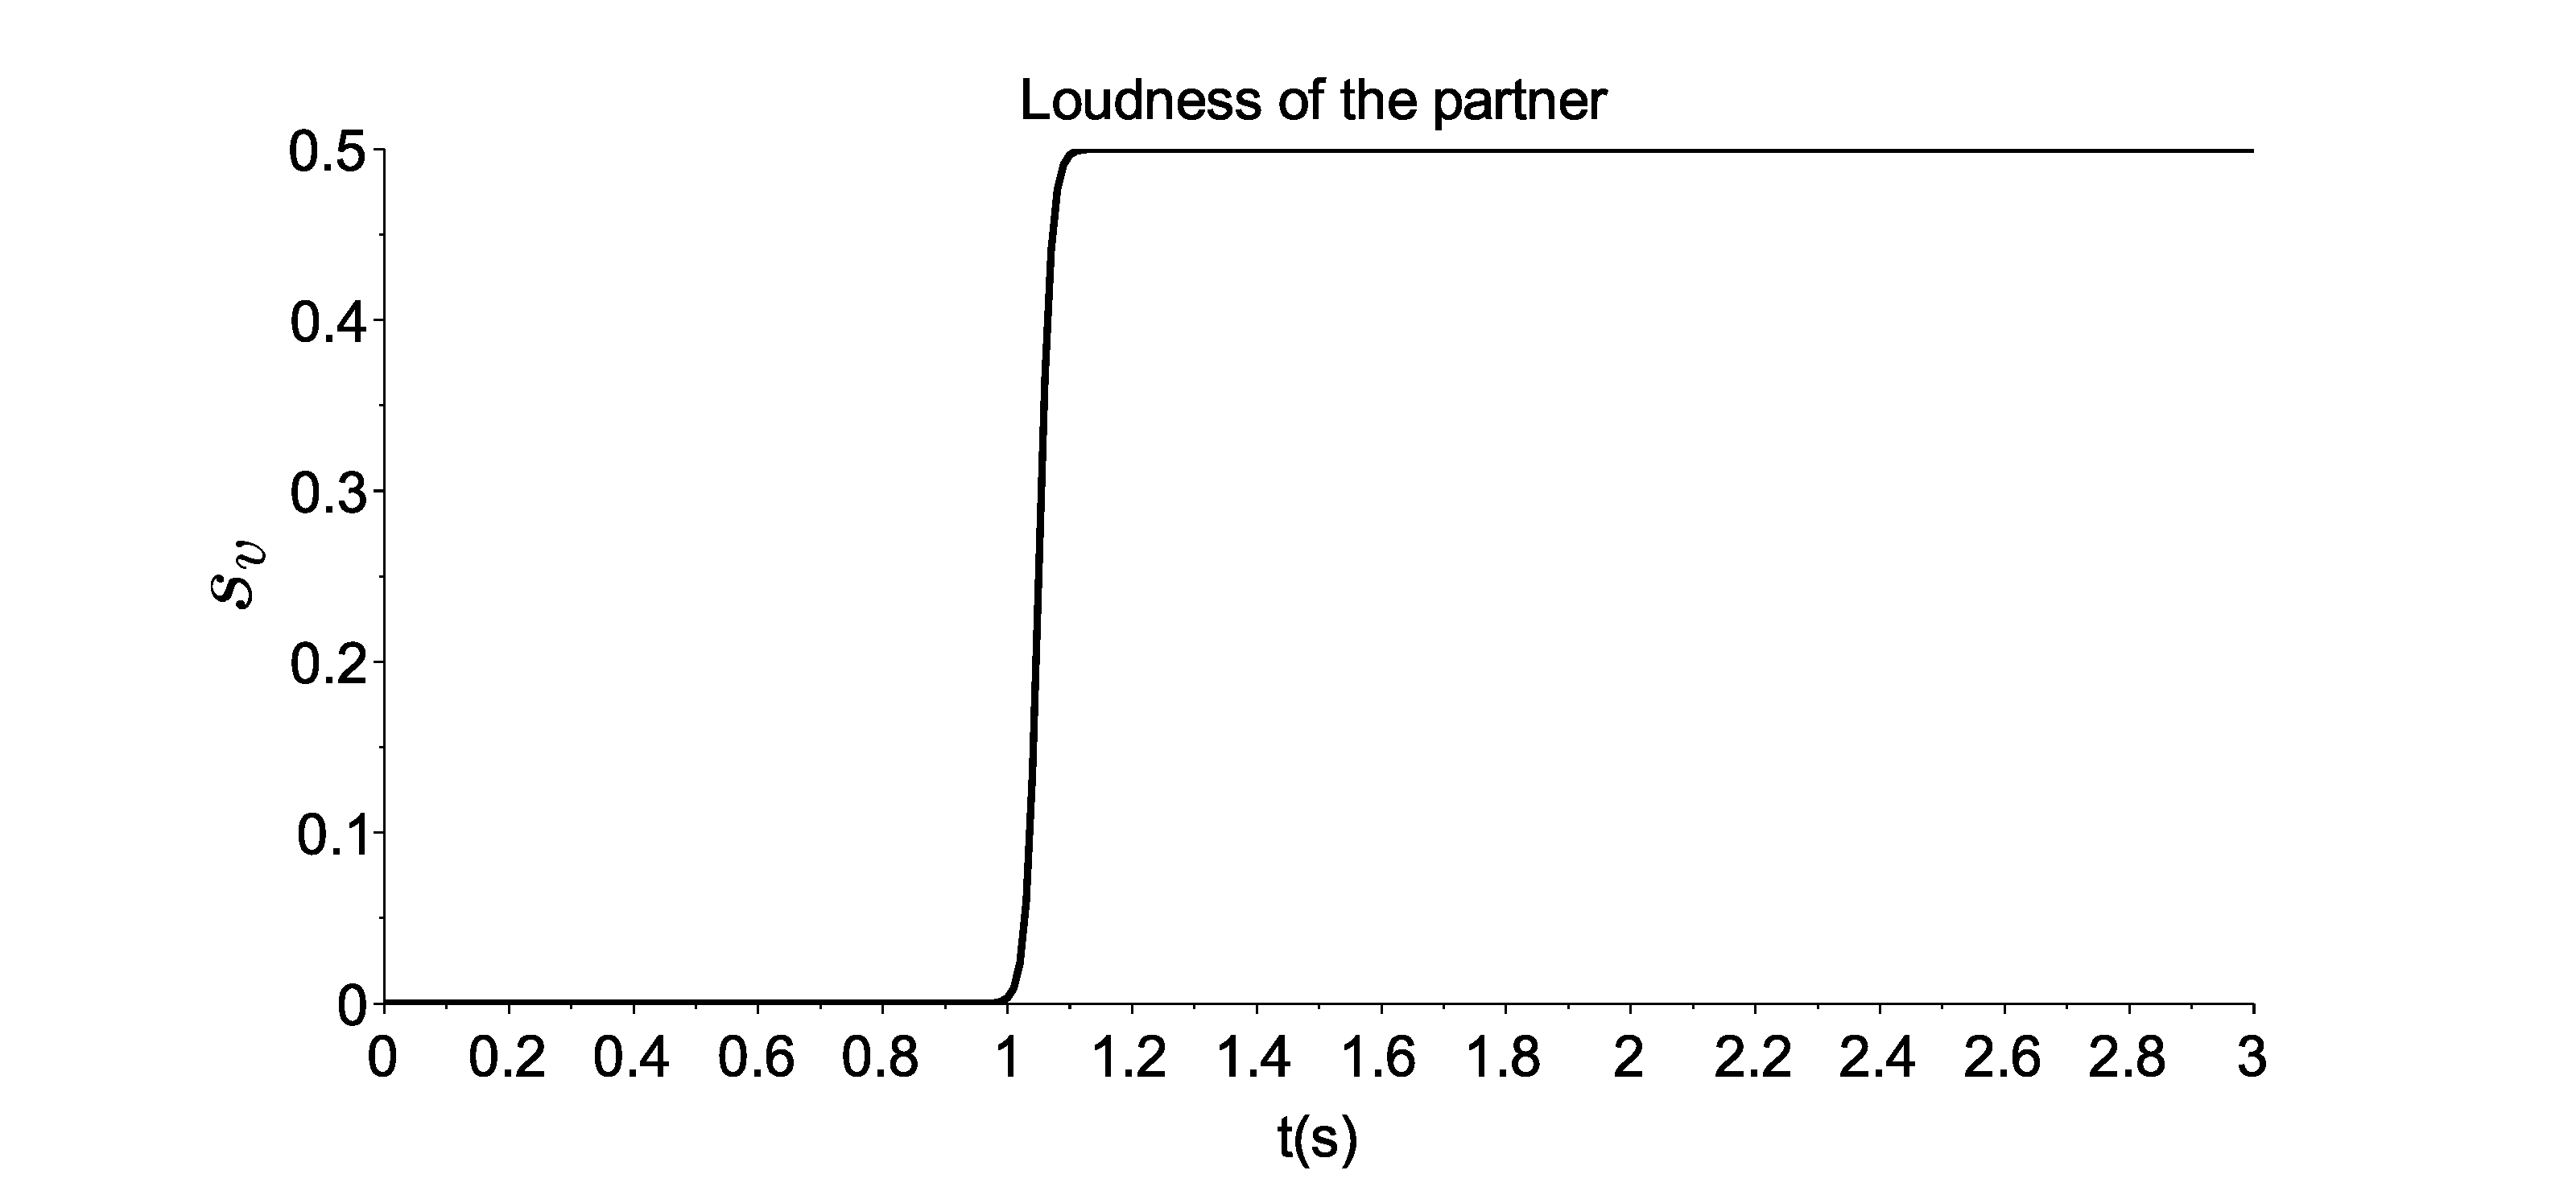
\includegraphics[width=\linewidth]{figure/loudness_simulated_partner.pdf}
  \caption{Illustrative simulation S1: variation of the voice loudness of the simulated user.}
  \label{fig-volume-user1}
\end{figure}

\begin{figure}%[b]
  \centering
  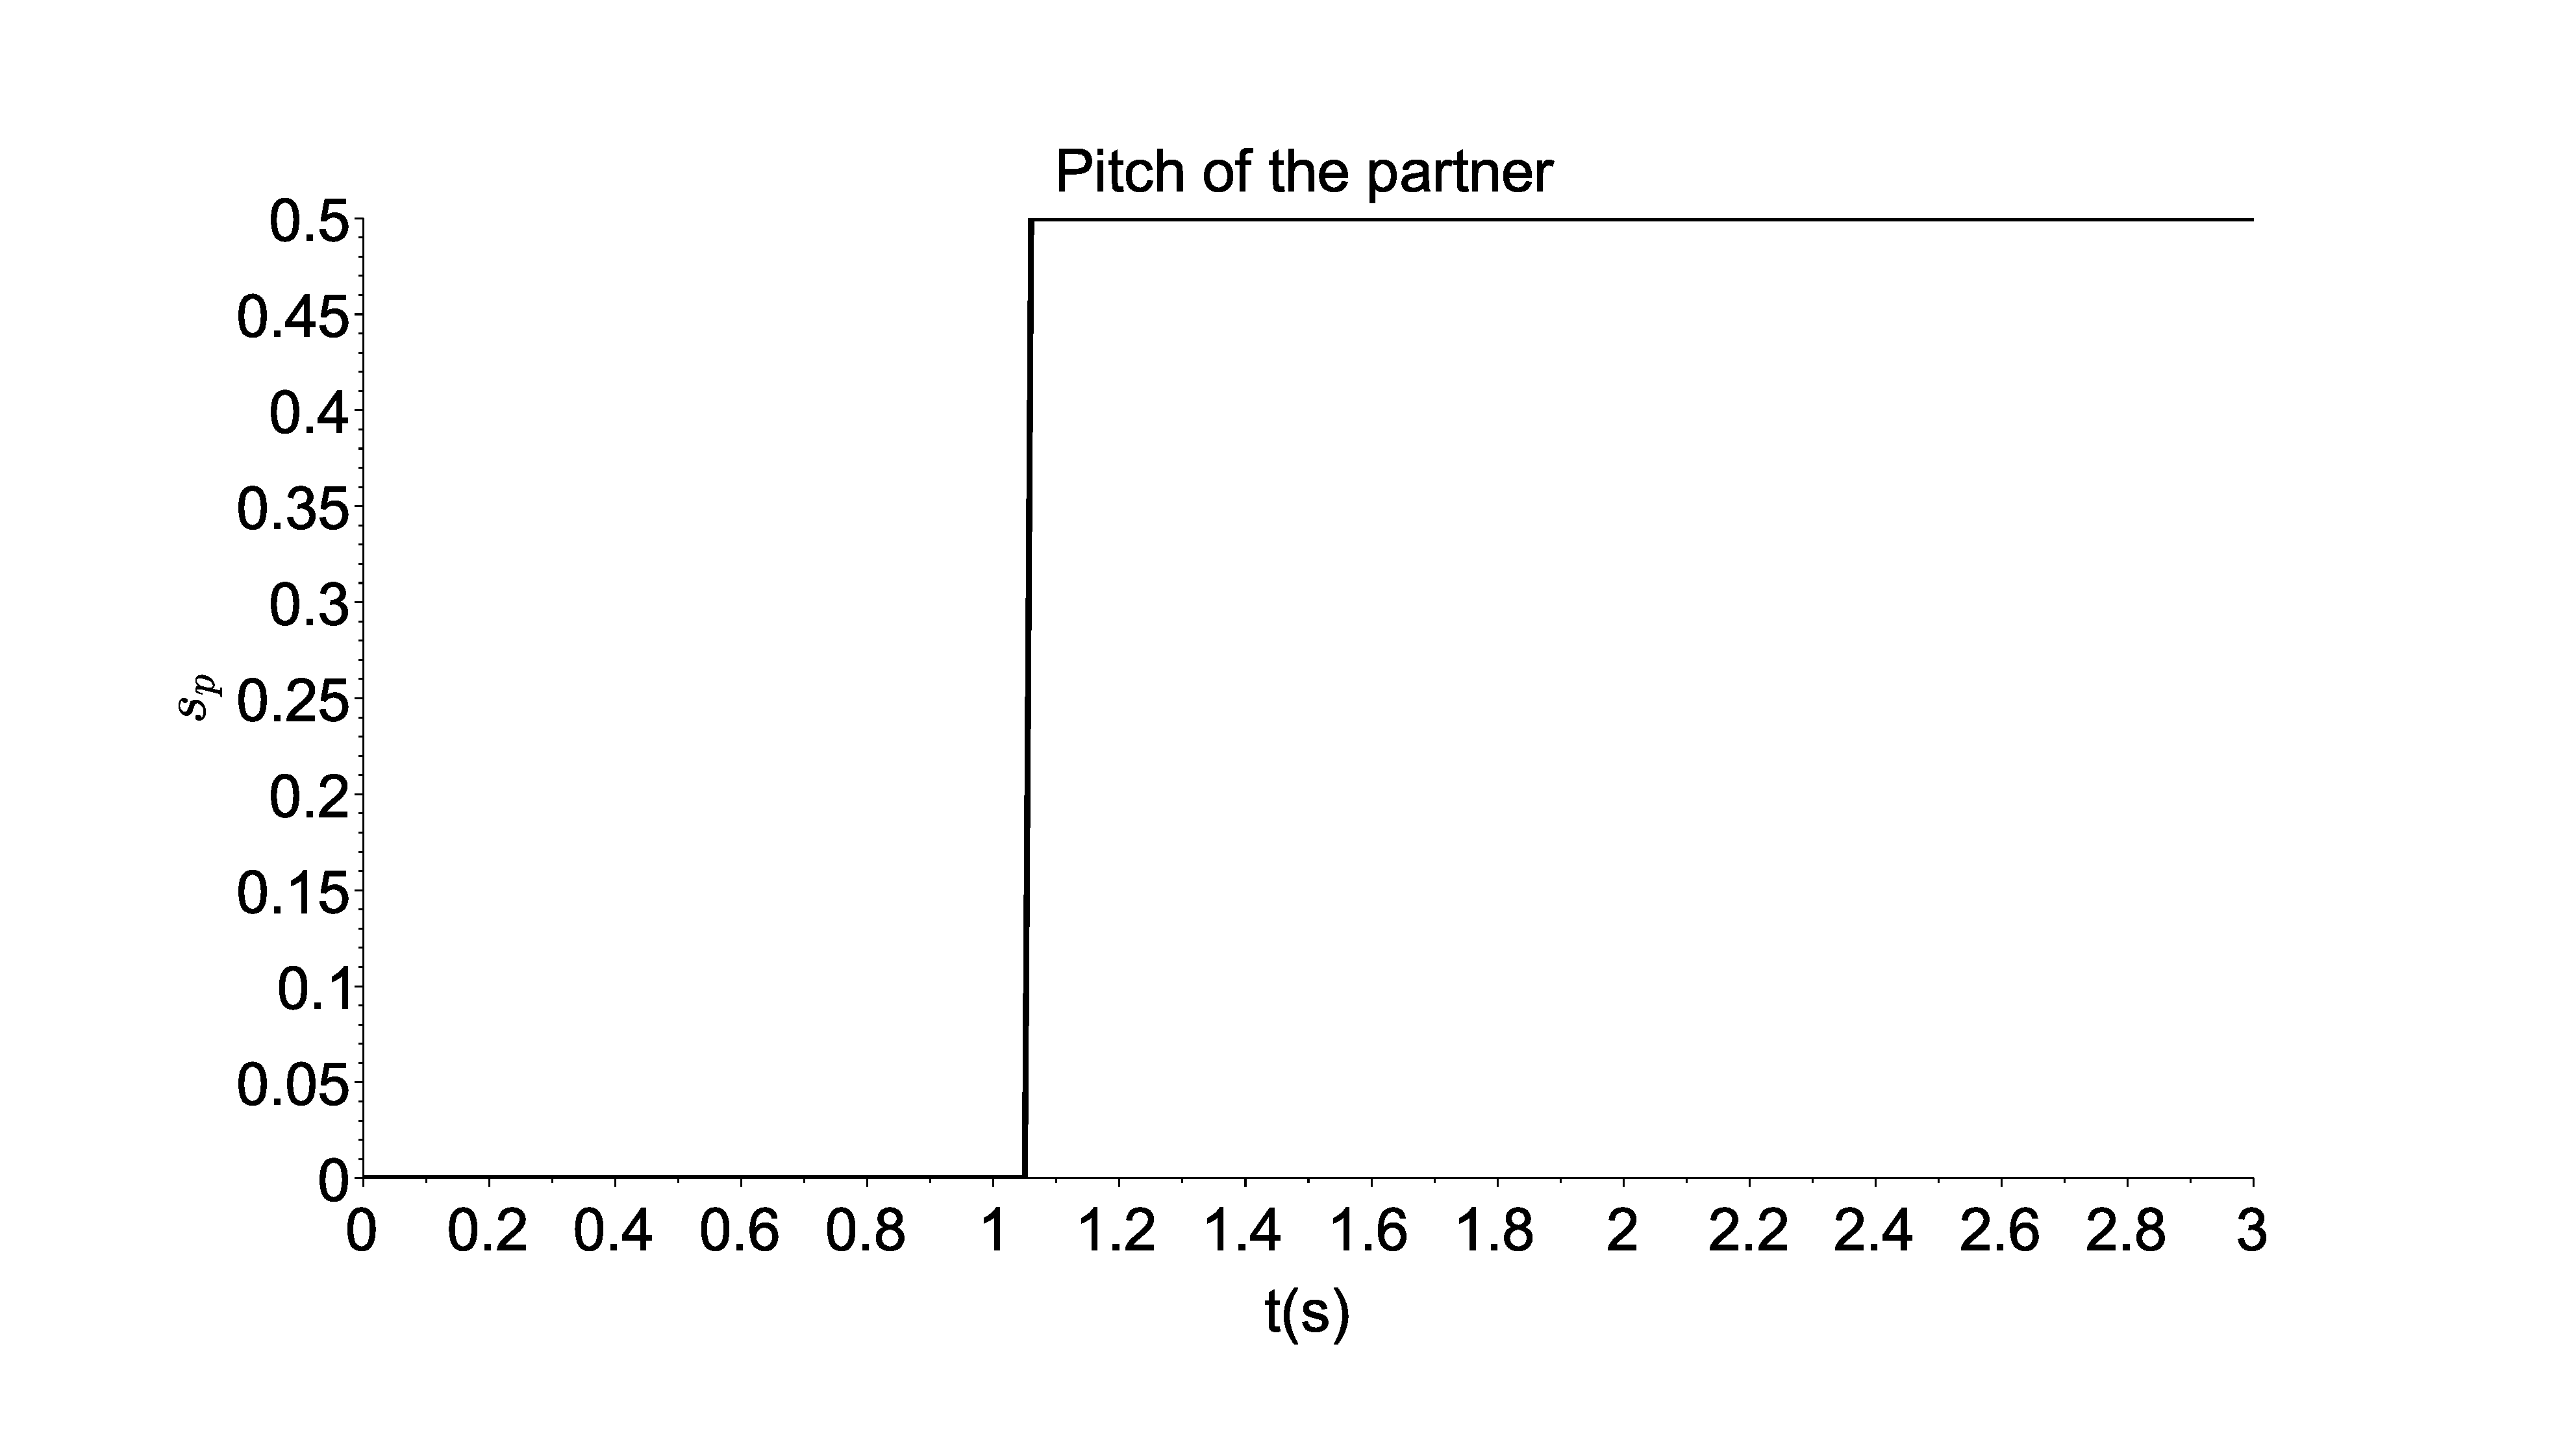
\includegraphics[width=\linewidth]{figure/Pitch_partenaire.pdf}
  \caption{Illustrative simulation S1: variation of the pitch of the simulated user.}
  \label{fig-pitch-user1}
\end{figure}

\begin{figure}
  \center
  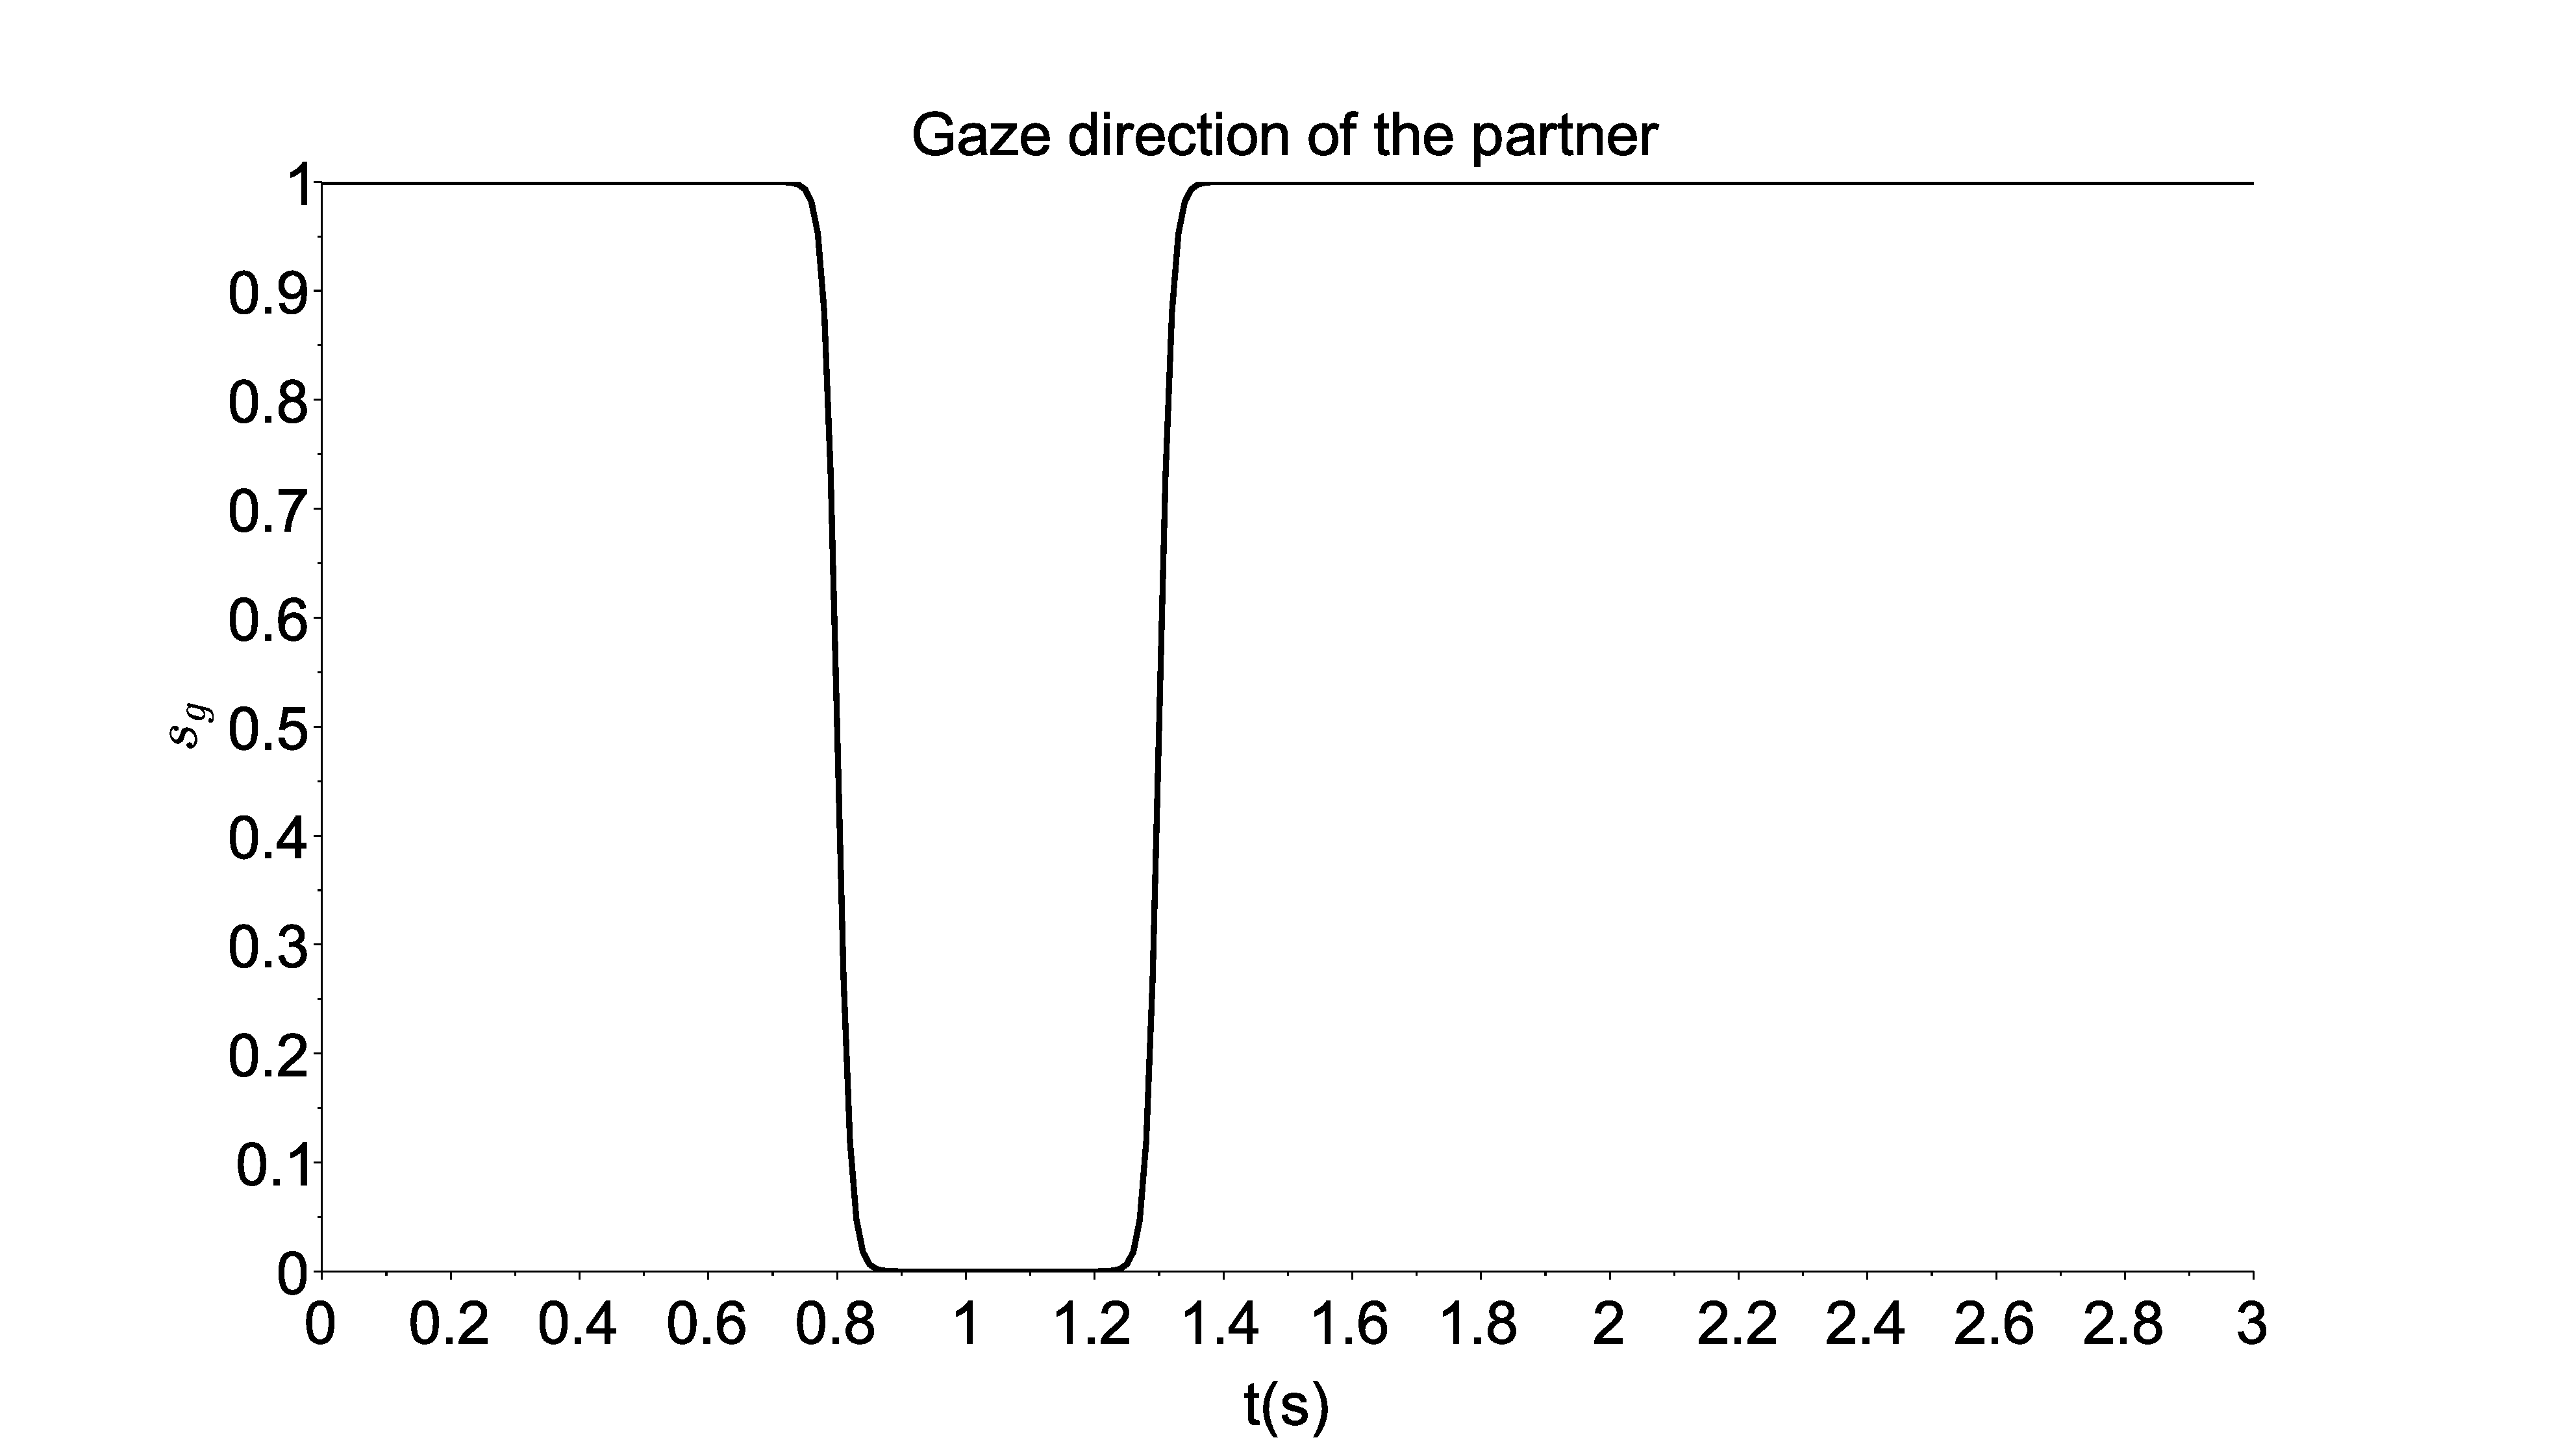
\includegraphics[width=\linewidth]{figure/Gaze_partenaire.pdf}
  % \end{subfigure}
  \caption{Illustrative simulation S1: variation of the gaze direction of the simulated user.}
  \label{fig-gaze-user1}
\end{figure}

\begin{figure}
  \centering
  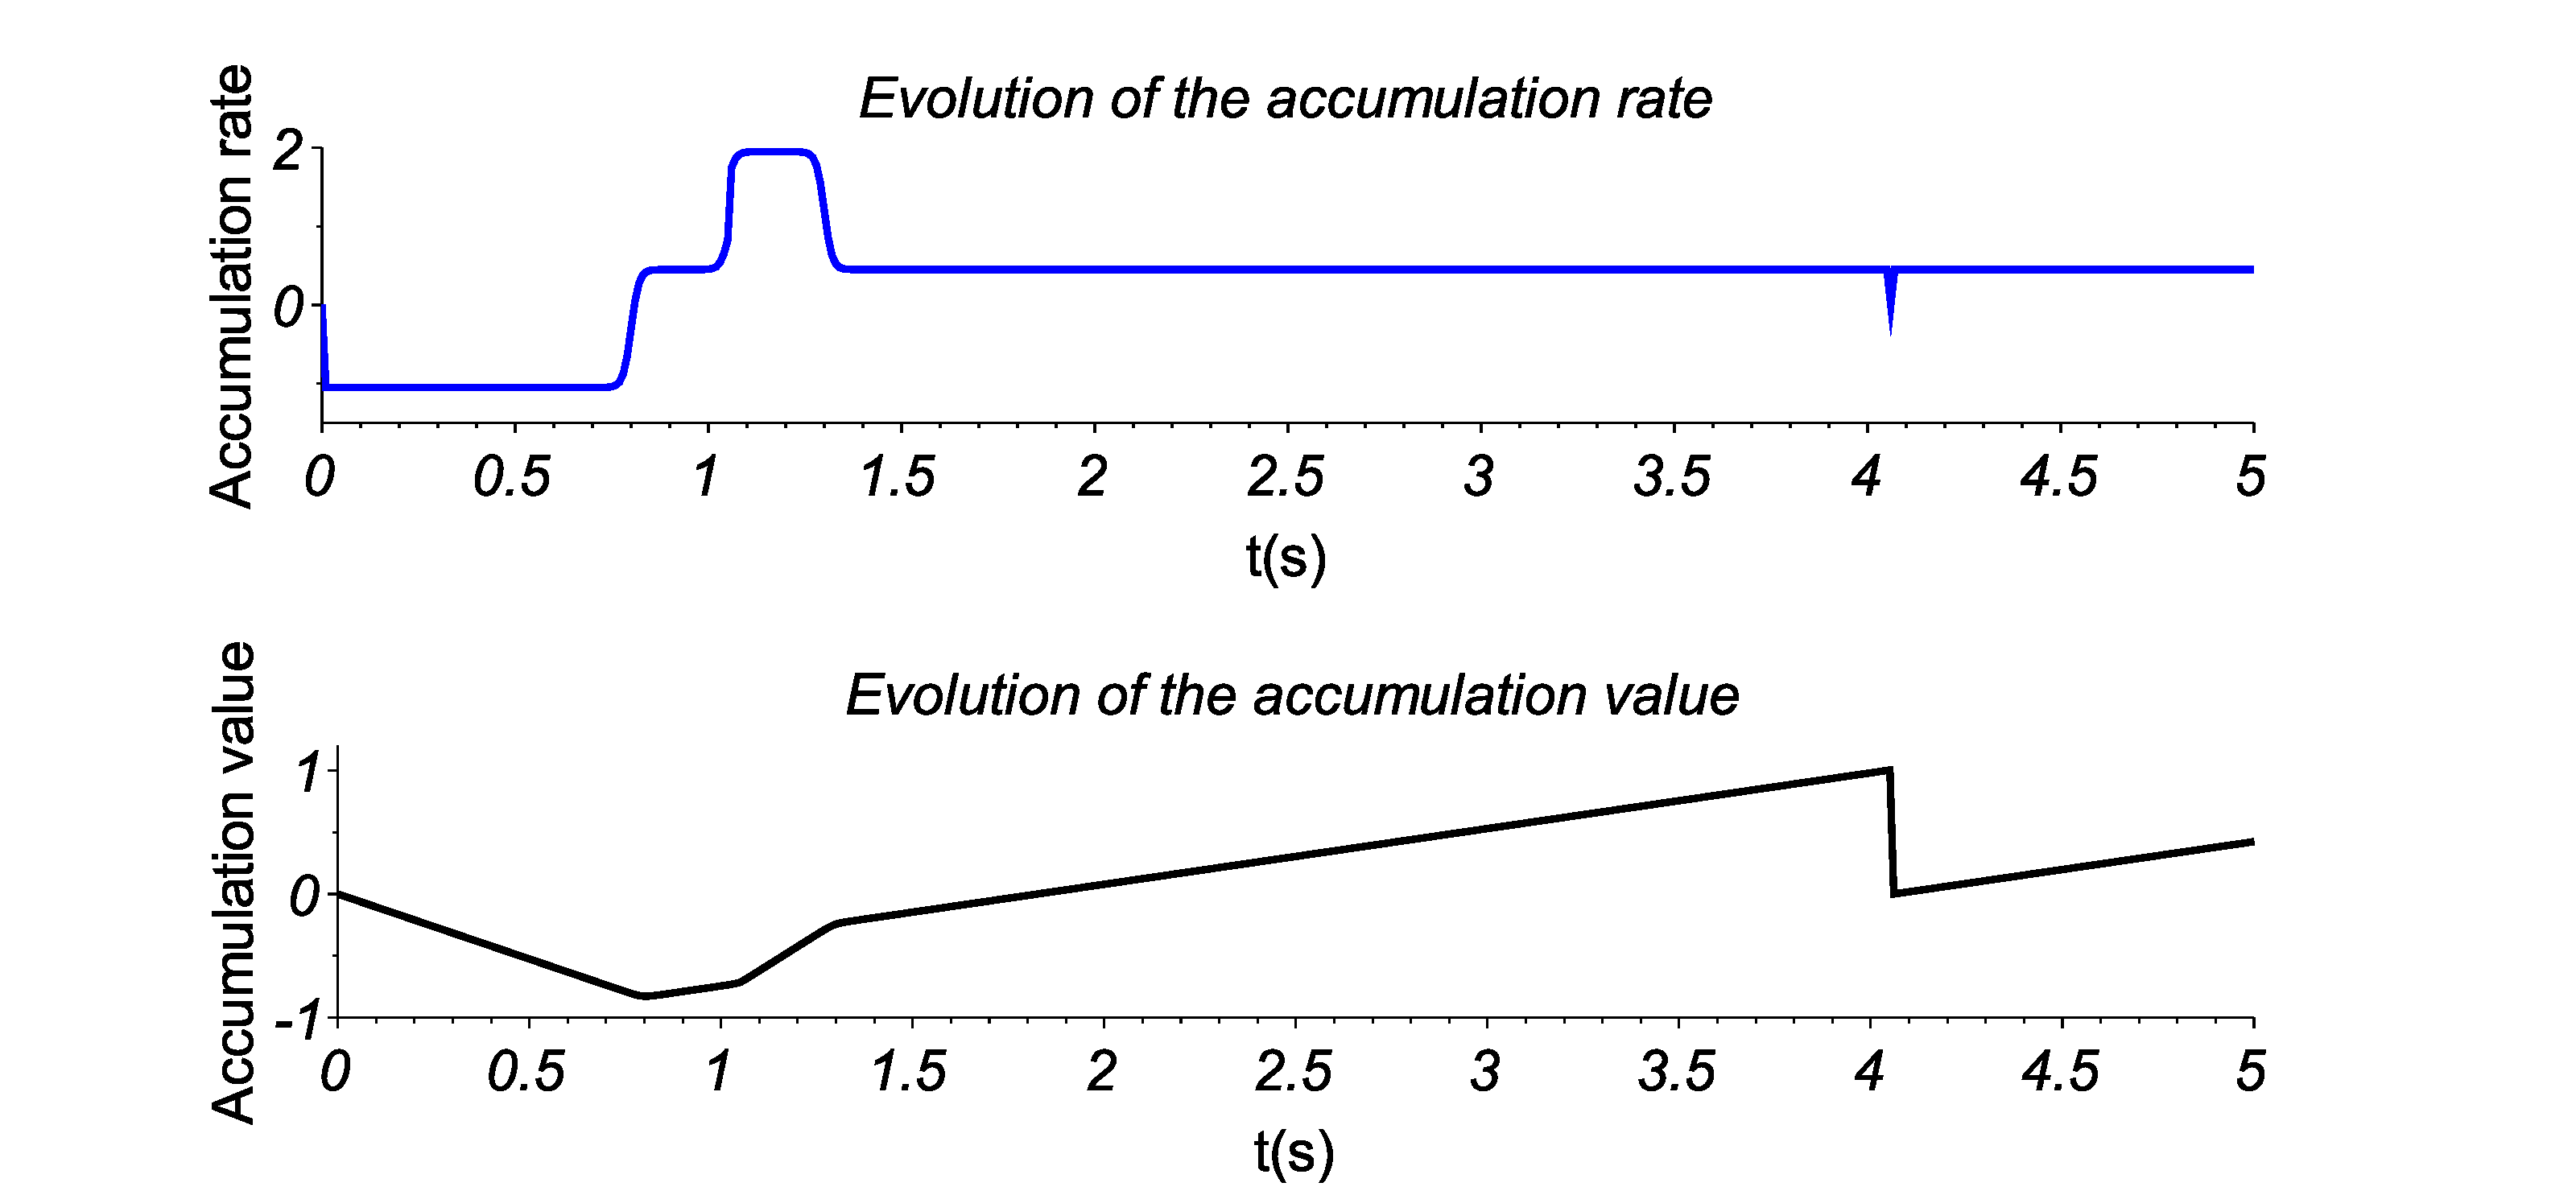
\includegraphics[width=\linewidth]{figure/illustration_ddm_speaker.pdf}
  \caption{Illustrative simulation S1: resulting dynamics of the perceptual decision-making process for the simulated speaker agent.}
  \label{acc_example}
\end{figure}

At the beginning of the scenario, the user did not produce any turn-taking signals, thus $\gamma(t)$ was decreasing, meaning that the agent was getting more and more confident about the user's intention to not claiming the turn. 

At $t=0.75~\text{s}$, the agent started to get some information about the user's willingness to take the turn (gaze avertion), thus the accumulation rate was positive. 
As soon as the user produced an additional turn-taking signal (starting to speak, resulting in a sudden increase in the pitch and volume of his voice), the accumulation rate raised to a higher value. 
After $=1.2~\text{s}$, the user's direction of gaze led the user to believe that the user did not want to take the turn, in contradiction with the information provided at the same time by the verbal channel (the user was actually speaking). Therefore the accumulation rate has fallen to an intermediate positive value. 
As a result, the agent accumulated information about the user's intention to effectively take the turn and $\gamma(t)$ reached the positive threshold ($\theta_{\gamma}^{+}=1$), leading it to be certain about the user's behavior. At this point ($t=4~\text{s}$), the agent made a definitive decision and it reset its perceptual decision-making process. 
Nevertheless, because the agent did not want to let the user taking the turn, it kept its current role, namely being the speaker. 

% As the user only and slightly increases its gesture production at the beginning, the accumulation value decreases towards the negative threshold $\theta_{\gamma}^{-}=-1$. 
% Then, as the user increases its gesture production and look away from the agent after approximately 750 ms, the accumulation rate varies to a positive value, but close to $0$, that results in an accumulation value that slightly increases, after which the user begins to speak after 1.1s. This sudden variation of the prosody descriptors strongly increases the accumulation rate, then the accumulation value rapidly converges towards the value $\theta_{\gamma}^{+}=1$, meaning that the agent is certain that the user is taking the turn. 

The  difference in the dynamics of the perceptual decision-making process, before and after $t=1.1~\text{s}$, illustrates the principle of additivity of the perceptual decision-making process, captured by Equation \ref{alpha_func}: the more signals the user produces
%The more the user produces signals,   
 the higher the accumulation rate and the faster the agent detects that the user is taking the turn. This additivity of the perceptual process has been reported for human conversations \citep{gravano_turn-taking_2011,hjalmarsson_additive_2011}. 

\subsubsection{Production of the communicative signals}

The second component of our theoretical model controls the continuous production of the verbal and nonverbal signals of the agent.
Following the principles of the behavioral dynamics formulated by \citep{warren_dynamics_2006}, each signal produced by the agent is controlled by a differential equation, representing the law of control of the agent's behavior. These equations have the following general shape: 

\begin{equation}
  \ddot{a_j}(t)= -b\times\dot{a_j}(t) - k_g \times(a_j(t) - f(m(t),\gamma(t)))
  \label{signal_control}
\end{equation}

$a_j(t)$ representing the current value of signal $j$, ($\ddot{a_j}(t)$ being the second derivative of the signal), $-b$ a damping term representing the intrinsic inertia of the agent to vary its signals, and $k_g\times(a_j(t)-f(m,\gamma))$ defining the value towards which the agent's signal is converging. In our theoretical model, each signal variable $a_j(t)$ is normalized within $ [0.0,1.0] $, $0.0$ representing the minimal value of the signal (no-signal or baseline), and $1.0$ the maximal value of the signal. The way these theoretical values are translated into realistic physical values depends on the nature of the signal and on the actuator used to execute the action corresponding to the signal produced. 
$k_g$ represents a stiffness parameter of the equation, the greater the value of $k_g$ the more the participant will rapidly vary its signal towards the final value of the equation. 
$f(m,\gamma)$ is a function that defines the attractor of the system. According to the sensorimotor coupling hypothesis (see section \ref{backgd}), the modulation of each signal is directly influenced by the motivation of the agent, $m$, and the accumulation value $\gamma$ provided by the perceptual decision-making component of our model.

%As an example showing how these equations are used to modulate the signals of the agent, 
\paragraph{Illustrative simulation S2.} Let's consider an agent currently being the speaker and modulating two prosodic signals ($v$ = loudness, $p$ = pitch) and its gaze direction, $g$. 
Like for the previous example, these variations are here theoretical.
The aim was not here to reproduce exactly the variations of the signal observed during human conversations, but to capture the dynamics of the signal productions, for instance that loudness and pitch tend to increase %and the speech rate to decrease 
during conflicting overlaps between partners, or to decrease during ends of turn. 

For each signal $j \in \lbrace p,v,g \rbrace$ produced by the agent, being the current speaker, we defined the following different equations $f_{j_{loc}}(m,\gamma)$, used in Equation \ref{signal_control}.
%According to Equation \ref{signal_control}, $f_p, f_v$ and $f_r$ are 
These functions control dynamically the value toward which each signal is varying at a given instant of time.

% Here are the new equations
\begin{equation}
\begin{array}{lcl}
f_{p_{loc}} & = &  \frac{1}{2}\Big( 1 - S(\gamma) \big( \gamma m S(-m) - S(m+\gamma)S(m) \big) \Big)
%0.5 -0.5 \times \gamma \times m \times S(-m) \times S(\gamma) - 0.5 S(m+\gamma) \times S(\gamma) \times S(m)\\
 %& = & \frac{1}{2}(1 - S(\gamma)\times\gamma \times m \times S(-m) - S(m+\gamma) \times S(m)))
\end{array}
\label{eq_speaker_pitch}
\end{equation}

\begin{equation}
f_{v_{loc}} = f_{p_{loc}}
\label{eq_speaker_volume}
\end{equation}

\begin{equation}
\begin{array}{lcl}
f_{g_{loc}}&=& \frac{1}{2}\Big( 1+\gamma m S(\gamma) \big(S(m) - S(-m)\big) \Big)\\
%& & 0.5 +0.5\times \gamma \times m \times S(\gamma) \times S(m) \\
%& & -0.5 \times \gamma \times m \times \times S(\gamma) \times S(-m) \\
%&=& \frac{1}{2}((1+\gamma \times m \times S(m) \times (S(\gamma) - \gamma \times m \times S(\gamma) \times S(-m))\\
\end{array}
\label{eq_speaker_gaze}
\end{equation}

\begin{equation}
S(x) = \frac{1}{1+e^{-10x}}
\label{eq_sigmoid}
\end{equation}

% \begin{equation}
% \left\lbrace
% \begin{array}{l c l}
% f_p(m(t),\gamma(t)) &=& \frac{1}{2}(1+S(\gamma(t))(S(-m(t)) - S(m(t)))\\
% f_v(m(t),\gamma(t)) &=& f_p(m(t),\gamma(t))\\
% f_r(m(t),\gamma(t))& =& \frac{1}{2}(1- S(\gamma(t)) \\
% S(x)&=&\frac{1}{1+e^{-5x}}
% \end{array}\right.
% \label{attr_foncs}
% \end{equation}

%$(m(t),\gamma(t))$ being the function defining how the final value of the pitch varies, 
%$f_v(m(t),\gamma(t))$ being the function defining how the final value of the loudness of the participant's voice varies
%and $f_r(m(t),\gamma(t))$ defining the variation of the final value of the speech rate. 

In these equations, we used the sigmoid function $S$ (Equation \ref{eq_sigmoid}) that permits to set to $0$ some terms, depending on the value of $\gamma(t)$ or $m(t)$ (when $x \gg 0$, $S(x)\approx 1$ and when $x \ll 0$, $S(x)\approx 0$). 
%The three functions have a quit similar behavior. 
For example for the control of the pitch, 
when $m(t) \gg 0$, Equation \ref{eq_speaker_pitch} reduces to $f_{p_{loc}}(m,\gamma) \sim \frac{1}{2}\big( 1-S(\gamma) \big)$, 
when $m(t) \ll 0$, $f_{p_{loc}}(m,\gamma) \sim \frac{1}{2}\big( 1 + S(\gamma)\big)$ 
and when $\gamma(t) \ll 0$, $f_{p_{loc}}(m,\gamma) \sim \frac{1}{2}$. 
%when $m(t) \gg 0$, the equation reduces to $f_v(m(t),\gamma(t)) \sim \frac{1}{2}(1-S(\gamma(t)))$, 
%when $m(t) \ll 0$, it becomes $f_v(m(t),\gamma(t)) \sim \frac{1}{2}(1 + S(\gamma(t))$ 
%and when $\gamma(t) \ll 0$, the equation becomes $f_v(m(t),\gamma(t)) \sim 0.5$. 
% ----

We set these functions such as, when the current speaker has a strong motivation to keep on speaking ($m(t) \ll 0$) and has accumulated enough cues indicating that the current listener is about to take the turn  ($\gamma(t) \gg 0$), the agent is expected to increase the loudness and the pitch of its voice to avoid its partner to take the turn, resulting in a conflicting overlap. 
%In such a situation, we also expect the speech rate to decrease, as observed by \citep{schegloff_overlapping_2000}.
Otherwise, when the current speaker's current goal is to leave the turn ($m(t) \gg 0$), it is expected to lower its loudness and pitch, even faster if the listener is starting to speak (all the signals are falling to 0).
%We defined these different functions such as when $m(t)<0$ and $\gamma(t)>0$ the loudness and the pitch increase, representing a conflicting situation, and the speech rate decreases following the observations made by \citep{schegloff_overlapping_2000}. When $m(t)>0$ and $\gamma(t)>0$ the loudness, the pitch and the speech rate decrease until $0$. 
Notice that setting $f_p = f_v$ is an approximation that makes the two signals to follow the same dynamics, according to the signs of $m(t)$ and $\gamma(t)$. 

Because our approach assumes the sensory-motor coupling of the two interacting agents, we have here to simulate the dynamic of its partner's behavior, as perceived by the agent.
For the sake of simplicity, we simulated the dynamic of the perceptual decision making using the following equation: $\gamma(t)=1-2e^{-t}$. 
It means that in the our simulated scenario, at the beginning the agent was certain that the listener is not claiming the turn ($\gamma(0) = -1$) and that the agent was rapidly accumulating some cues in the current listener's behavior indicating the willingness of the listener to take the turn. 

%Based on these equations, 
Figure \ref{demo_simu_l1} shows how the agent varied its prosodic signals when it was strongly motivated to keep on speaking ($m=1$).
As the accumulation $\gamma(t)$ increased, the resulting values of $f_v$ and $f_p$ increased towards $1$ and $f_g$ decreased towards $0$. 
Accordingly, the theoretical loudness and pitch of the agent raised to their maximum values (as expected during a conflicting overlap where the speaker tries to keep its role, and thus is modulating its signals production) in reaction to the listener's behavior that was trying to take turn. 

%We simulated a positive variation of the accumulation value from $-1$ to $1$ according to equation $\gamma(t)=1-2e^{-t}$. 

\begin{figure}
  \centering
  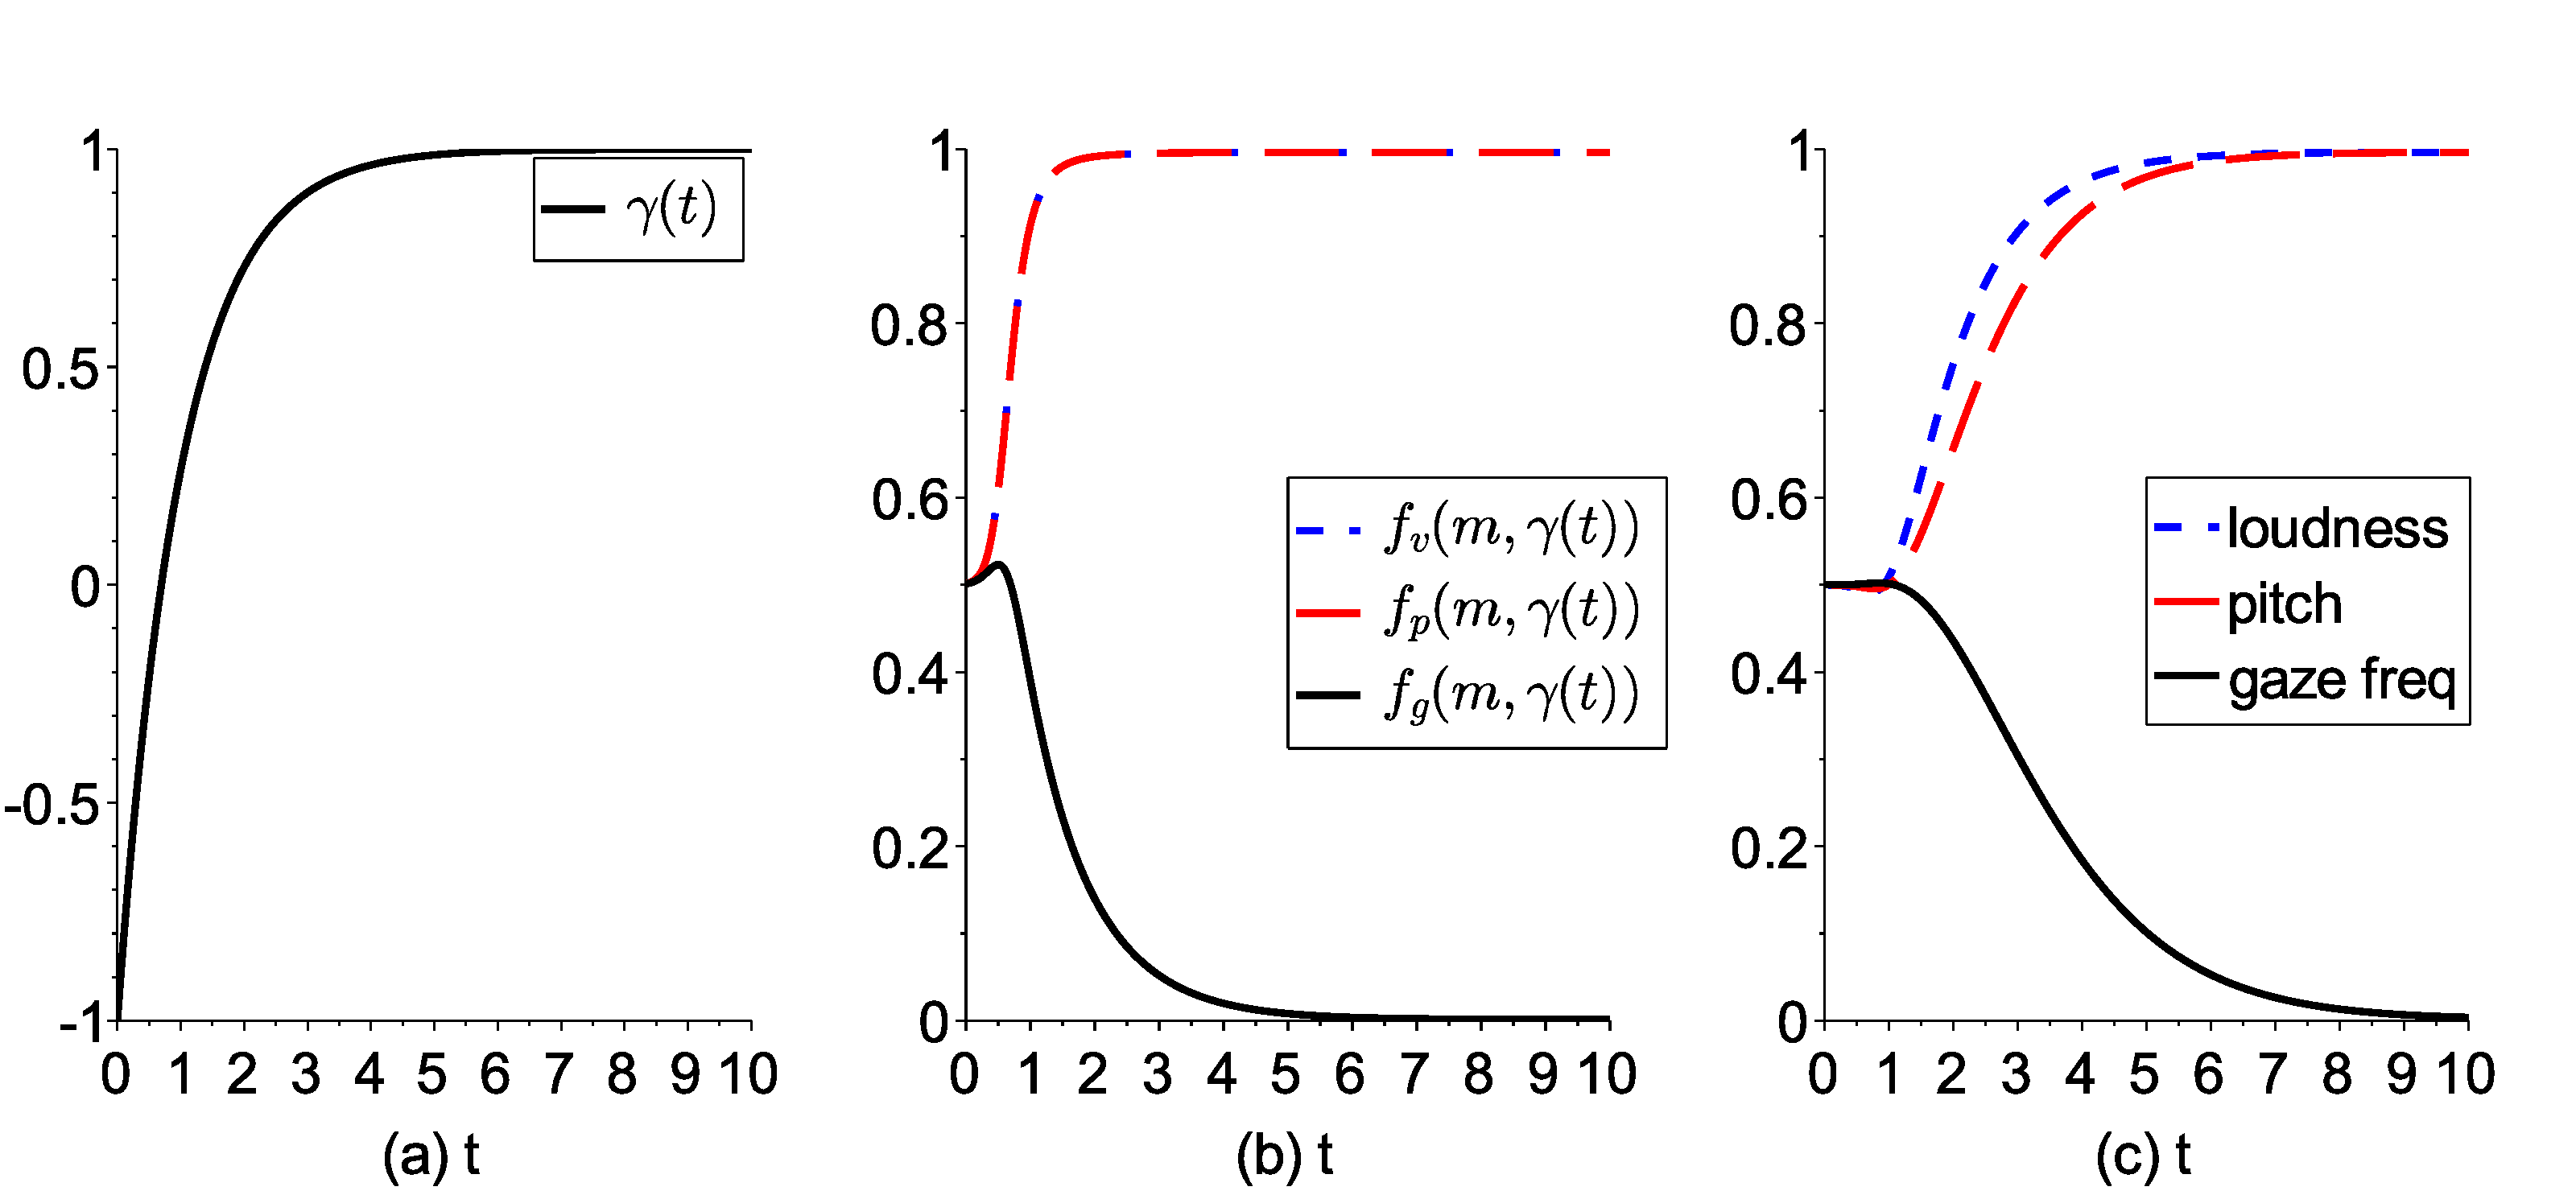
\includegraphics[width=\linewidth]{figure/signals_simu_s2a.pdf}
  \caption{Illustrative simulation S2: time series of the simulated speaker's signal productions. (a) simulation of the agent's perceptual decision-making process (value of $\gamma$). (b) the variations of $f_v(m,\gamma)$, $f_p(m,\gamma)$, $f_r(m,\gamma)$ . (c) resulting  signal productions. Case of an agent with a very strong motivation to keep being the current speaker ($m=-1.0$).}
  \label{demo_simu_l1}
\end{figure}

To illustrate how the agent's motivation impacts the dynamics of the signal production, we simulated the same scenario but with a speaker motivated to yield the turn ($m(t)=1$). As illustrated on Figure \ref{demo_simu}, in this case, $f_v$ and $f_p$ both decreased towards $0$, leading to a variation of the theoretical loudness and pitch towards $0$, illustrating a situation where the agent yielded the turn as it also perceived that the listener was taking the turn. 

\begin{figure}
  \centering
  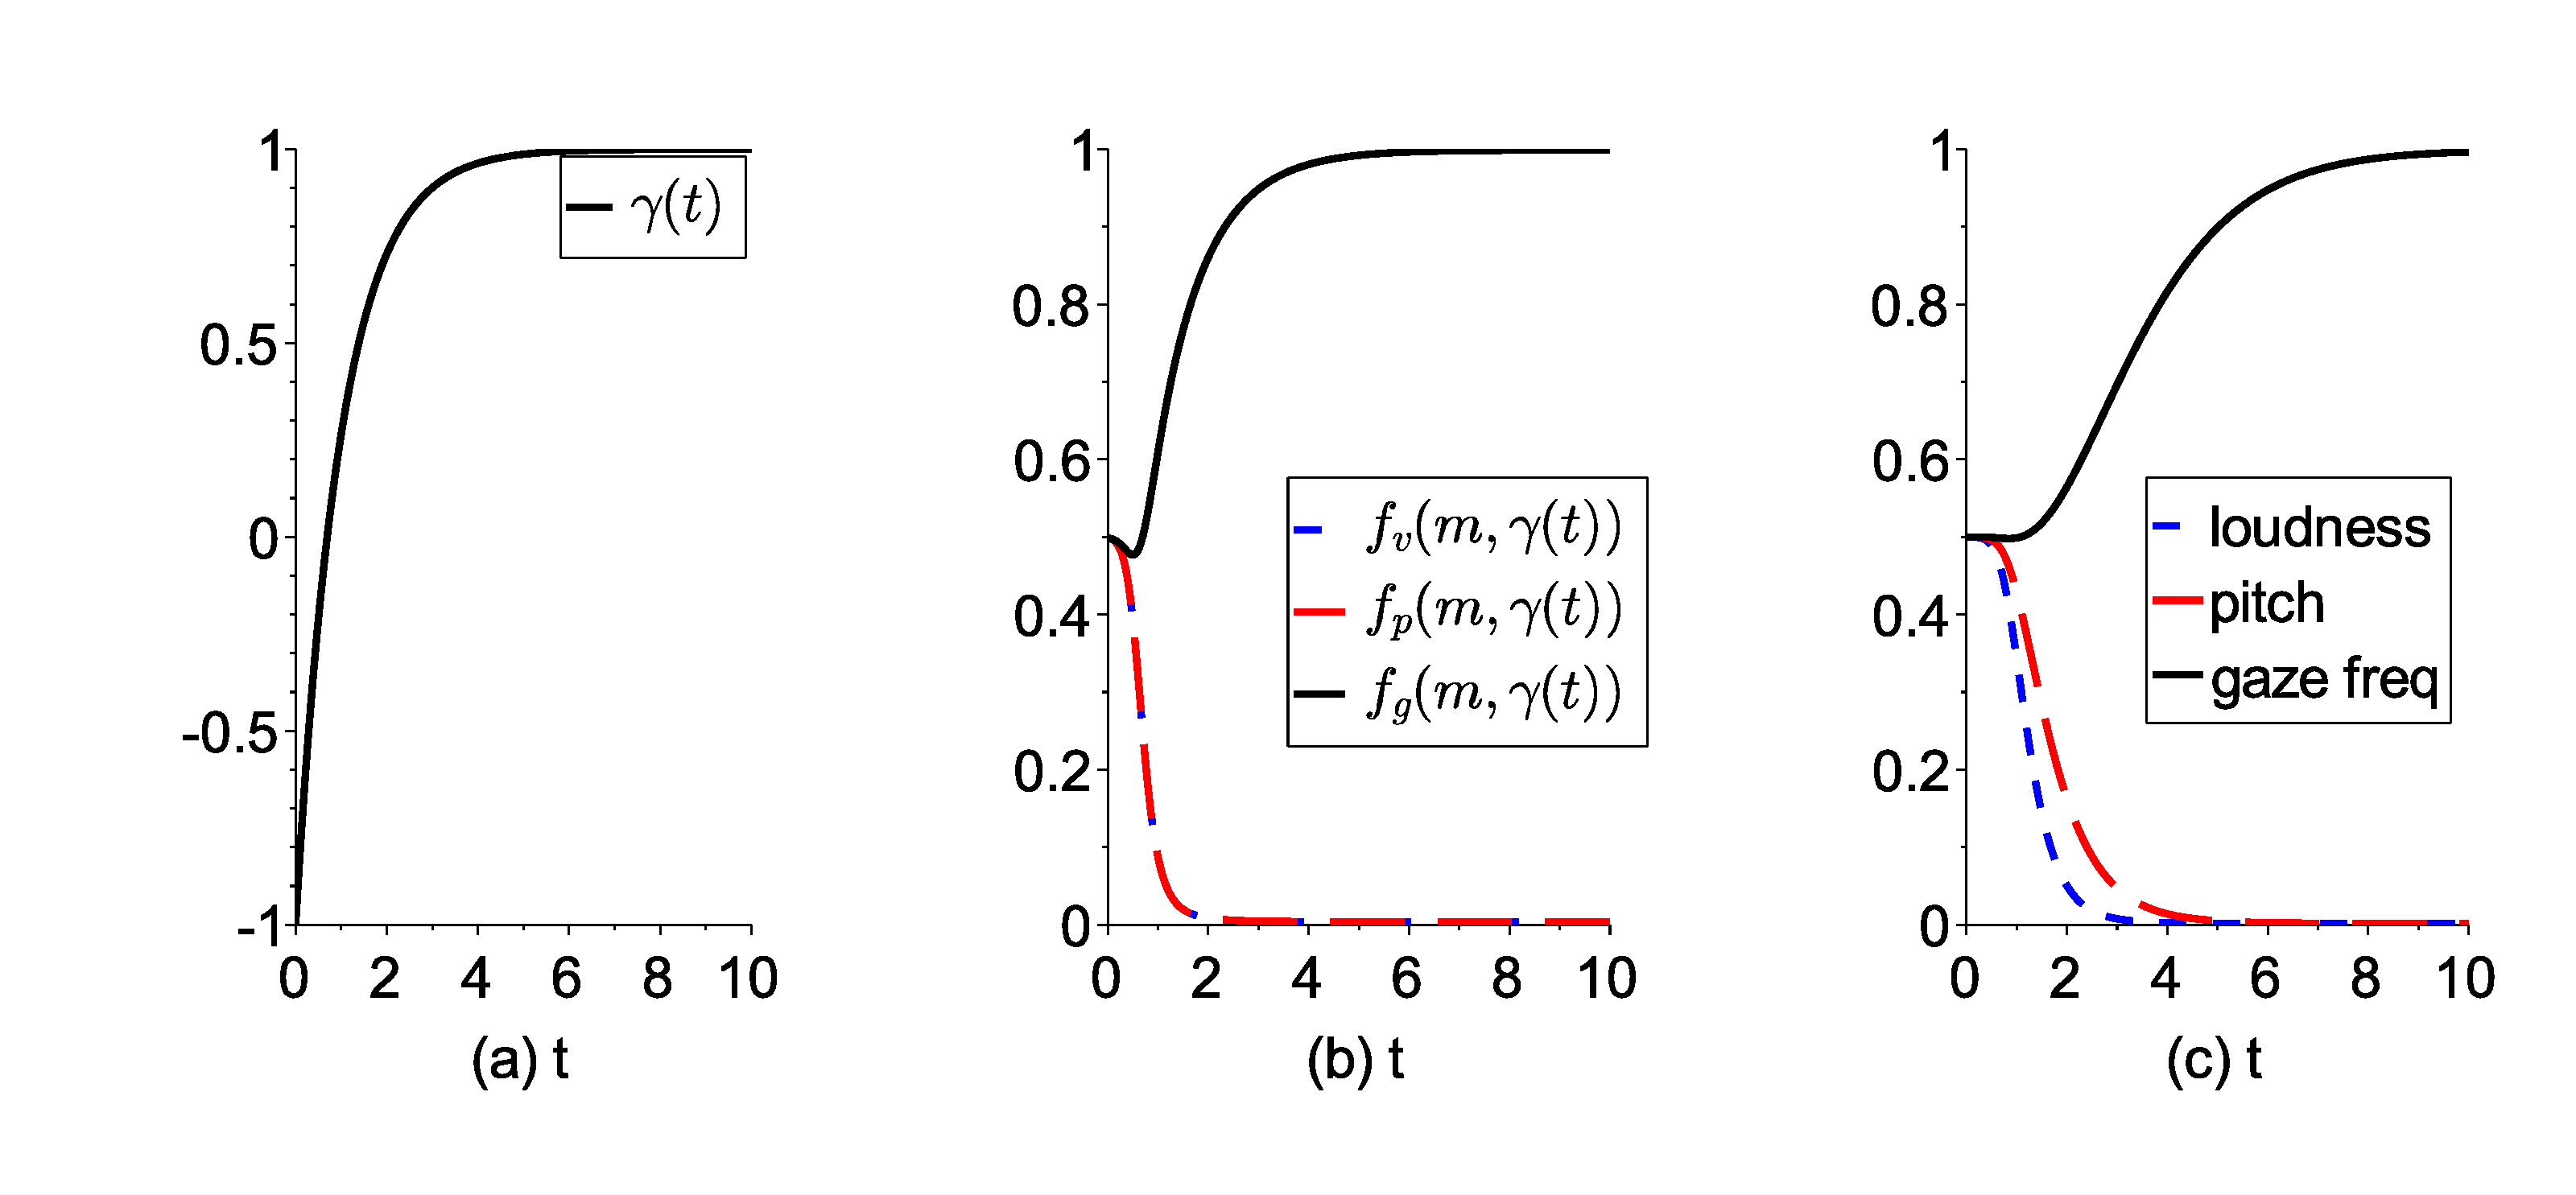
\includegraphics[width=\linewidth]{figure/signals_simu_s2b.pdf}
  \caption{Illustrative simulation S2: time series of the simulated speaker's signal productions. (a) simulation of the agent's perceptual decision-making process (value of $\gamma$). (b) the variations of $f_v(m,\gamma)$, $f_p(m,\gamma)$, $f_r(m,\gamma)$ . (c) resulting  signal productions. Case of an agent with a very strong motivation to leave the turn ($m=1.0$).}
%  \caption{Illustration of a simulation with a simulated variation of the accumulation value. The variation of $f_v(m,\gamma)$, $f_p(m,\gamma)$, $f_r(m,\gamma)$ is illustrated on the middle figure, and the variation of actions on the right figure. In this example the agent has a motivation $m_{sp}=1.0$.}
  \label{demo_simu}
\end{figure}
